\documentclass[
    12pt, % Schriftgröße
    ngerman, % für Umlaute, Silbentrennung etc.
    a4paper, % Papierformat
    oneside, % einseitiges Dokument
    headings=big, % Größe der Überschriften verkleinern
    listof=totoc, % Verzeichnisse im Inhaltsverzeichnis aufführen
    bibliography=totoc, % Literaturverzeichnis im Inhaltsverzeichnis aufführen
    index=totoc, % Index im Inhaltsverzeichnis aufführen
    captions=tableheading, % Beschriftung von Tabellen unterhalb ausgeben
    final % Status des Dokuments (final/draft)
    %toc=chapterentrywithdots %Inhaltsverzeichnis mit Punkten
    sectionentrydots=true,
    toc = bibliography,
]{scrartcl}
%scrartcl -> Basis der Vorlage = Koma Script

%Allgemeine Pakete
\usepackage[utf8]{inputenc} 
\usepackage[ngerman]{babel}                         %Landessprache Deutsch
\usepackage[T1]{fontenc}                            %Schriftformatierung


% Graphik- und Tabellenpakete
\usepackage[pdftex]{graphicx}                       %Implementierung Grafiken
\graphicspath{{img/} }                              % Bildordner
\usepackage{subfig}                                 % Mehrere Graphiken nebeneinander
\usepackage{tabularx}                               %Tabellenpaket

%Tabellen für Formeln und Gleichungen
\usepackage{amsmath}


%Hyperlinks (erst am Ende aktivieren)
%\usepackage{hyperref}                              %Erstellen von Hyperlinks
%\usepackage[figure]{hypcap}                        %Hyperlinks für Abbildungen


%Schriftdarstellung und Textoptimierung 
\usepackage{mathptmx}               % Times New Roman
\usepackage{microtype}              % Blocksatzbildung
\hyphenation{De-zi-mal-tren-nung}   % Deutsche Zeilenbrüche
\usepackage{color}                  % Möglichkeit zum Verwenden von Farben
\usepackage{lmodern}                % bessere Fonts
\usepackage{relsize}                % Schriftgröße relativ festlegen
\usepackage{blindtext}              %Packet Blindtext zum Einfügen von sinnlosen Text


% Pakete für Geometrie und Abstände
\usepackage{geometry} %zunächst auf Standardeinstellungen belassen...
\usepackage{setspace} 



%Verzeichnispakete 
\usepackage[automark]{scrlayer-scrpage}             % Kopf und Fußzeile
\usepackage[printonlyused,withpage]{acronym}        % Abkürzungsverzeichnis



%Schriftarten von Section, Chapter, Text etc. einstellen, Format Inhaltsverzeichnis
\renewcommand{\rmdefault}{ptm}
\renewcommand{\sfdefault}{phv}
\renewcommand\familydefault{\rmdefault}
\addtokomafont{section}{\rmfamily\mdseries\Large \hspace*{-0.2cm}\vspace{-10pt}}
\addtokomafont{subsection}{\normalfont\large\rmfamily\bfseries\hspace*{-0.2cm}\vspace{-10pt}}
\addtokomafont{sectionentry}{\rmfamily\mdseries\large \hspace{-10pt}\vspace{-5pt}}
\newcommand*{\smalltocentry}[1]{\normalfont #1}% To setup the small ToC entries (see \RedeclareSectionCommand[…]{section})
\RedeclareSectionCommand[beforeskip=0pt,afterskip=\baselineskip,afterindent=false]{section}
\RedeclareSectionCommand[beforeskip=0pt,afterskip=\baselineskip,afterindent=false,tocentryformat=\smalltocentry]{subsection}

%Formelverzeichnis erstellen
\DeclareNewTOC[%
  counterwithin=chapter,
  %indent=0pt,% kein Einzug im Verzeichnis
  %hang=2em,% Einzug für den Text im Verzeichnis
  name=equation,
  type=xequation,
  nonfloat]{loe}

\AtBeginDocument{%
  \newcaptionname{ngerman}\xequationname{Formel}%
  \newcaptionname{ngerman}\listxequationname{Formelverzeichnis}%
}




%\KOMAoptions{toc=chapterentrydotfill}

%Formatierung des Tabellen/Abküerzungsverzeichnis anpassen
%\usepackage{tocloft}
%\renewcommand{\cftfigpresnum}{Abbildung. }
%\renewcommand{\cfttabpresnum}{Tabelle. }

%\renewcommand{\cftfigaftersnum}{:}
%\renewcommand{\cfttabaftersnum}{:}

%\setlength{\cftfignumwidth}{2cm}
%\setlength{\cfttabnumwidth}{2cm}

%\setlength{\cftfigindent}{0cm}
%\setlength{\cfttabindent}{0cm}

%\renewcommand{\figurename}{Abb.}
%\renewcommand{\tablename}{Tab.}


%\renewcommand{\cftfigpresnum}{Abb. }
%\settowidth{\cftfignumwidth}{Abb. 10\quad}
%\setlength{\cftfignumwidth}{2cm}




% Kopf- und Fußzeile der ersten Seiten (Paket scrlayer-scrpage)
\pagestyle{scrheadings}
\clearmainofpairofpagestyles{}  % alle Felder leeren
%\ihead{}\chead{}\chead{}
\ohead{\pagemark}               % Seitenzahl oben rechts



\begin{document}
\pagestyle{empty}
\begin{center}
\begin{tabular}{p{\textwidth}}
\begin{center}
\large {Private Fachhochschule für Wirtschaft und Technik \\
Bachelor of Engineering\\
Ausbildungsbetrieb: DIL Engineering GmbH}
\end{center}
\\
\begin{center}

\includegraphics[scale=1]{img/PHWT-Logo.jpg}
\end{center}
\\
\\
\begin{center}
\large{Praxistransferbericht zum Thema:}
\end{center}
\\
\begin{center}
\Large{Auslegung eines Druckbehälters nach Merkblatt AD2000}
\end{center}

\begin{center}
Beschreibung 1\\
Beschreibung 2
\end{center} \\
\begin{center}
vorgelegt von: 
\end{center}

\begin{center}
    \begin{tabular}{lll}
        \textbf{Steffen Specker:} & & Matrikelnr. 172897\\
        \end{tabular} 
\end{center}
\\
\\
\\
\begin{center}
\begin{tabular}{lll}
\textbf{Prüfer:} & & Herr Kray\\
\textbf{Abgabedatum:} & & 31.07.2022\\
\end{tabular}
\end{center}

\end{tabular}
\end{center}




%\hypersetup{pageanchor=true} %Hyperlinks erstellen
\pagenumbering{Roman}


%Absätze einstellen
\newgeometry{left=4cm, right=2cm, top=2cm}
\setlength{\parindent}{0cm}                     % Einrücken des Textes bei neuem Absatz
\setlength{\parskip}{0.5cm}                     % Vertikaler Abstand der Absätze
\doublespacing{}                                % Zeilenabstand

% Seitenränder für das Textdokument einstellen
\setlength{\headheight}{1.5cm}                  % Höhe Kopfzeile
\setlength{\voffset}{2.5cm}                     % Abstand Oberer Rand - Textfeld
\setlength{\topmargin}{-4.5cm}                  % Abstand Oberer Rand - Text oben
\setlength{\headsep}{0.5cm}                     % Abstand Kopfzeile - Text oben 
\setlength{\footskip}{2cm}                      % Abstand Fußzeile - Text unten
\setlength{\footheight}{1.5cm}                  % Höhe Fußzeile
%Abstand Gleitumgebungen zum Text
\setlength{\intextsep}{12pt}
\setlength{\textfloatsep}{12pt}

\addcontentsline{toc}{section}{Inhaltsverzeichnis}
\tableofcontents
%\setcounter{secnumdepth}{2}

\newpage
\listoftables % Tabellenverzeichnis
\vspace{2cm}
\listoffigures  %Abbildungsverzeichnis
\vspace{2cm}
\section*{Abkürzungsverzeichnis} 
\addcontentsline{toc}{section}{Abkürzungsverzeichnis} 

\begin{acronym}[Bash]
\acro{KDE}{K Desktop Environment}
\acro{dr}[Dr.]{Doktor}
\acroplural{dr}[Dres.]{Doktoren}
\acro{SQL}{Structured Query Language}
\acro{Bash}{Bourne-again shell}
\acro{JDK}{Java Development Kit}
\acro{VM}{Virtuelle Maschine}
\acro{I2C}[I²C]{Inter-Integrated Circuit}
\end{acronym}


\vspace{2cm}


%\section*{Formelverzeichnis} 
%\addcontentsline{toc}{section}{Formelverzeichnis} 
%\renewcommand{\listtablename}{}


\cleardoublepage{}


%Ab hier beginnt das eigentliche Dokument

\newpage
\pagenumbering{arabic}
\ofoot{\thepage}
\ihead{}
\chead{}
\ohead{}



\section{Einführung in das Thema}

This will be an empty chapter
Vor Jahren waren \ac{KDE} die größten Vermittler der Welt. \\
Des lässt sich auch an xx feststellen. Der Mehrwert Bla Bla \blindtext\par


\blindtext{}

\subsection{Unterkapitel}
\blindtext{}
\subsection{Noch eins}
\subsection{Ein weiteres}

\newpage

\section{Grundlagen der Sterilisation und Rahmenbedingungen für die Konstruktion eines Dampfdruckbehälters}
\blindtext[1]\par\blindtext[1.5]\par

\begin{figure}[htb]
    \centering  
    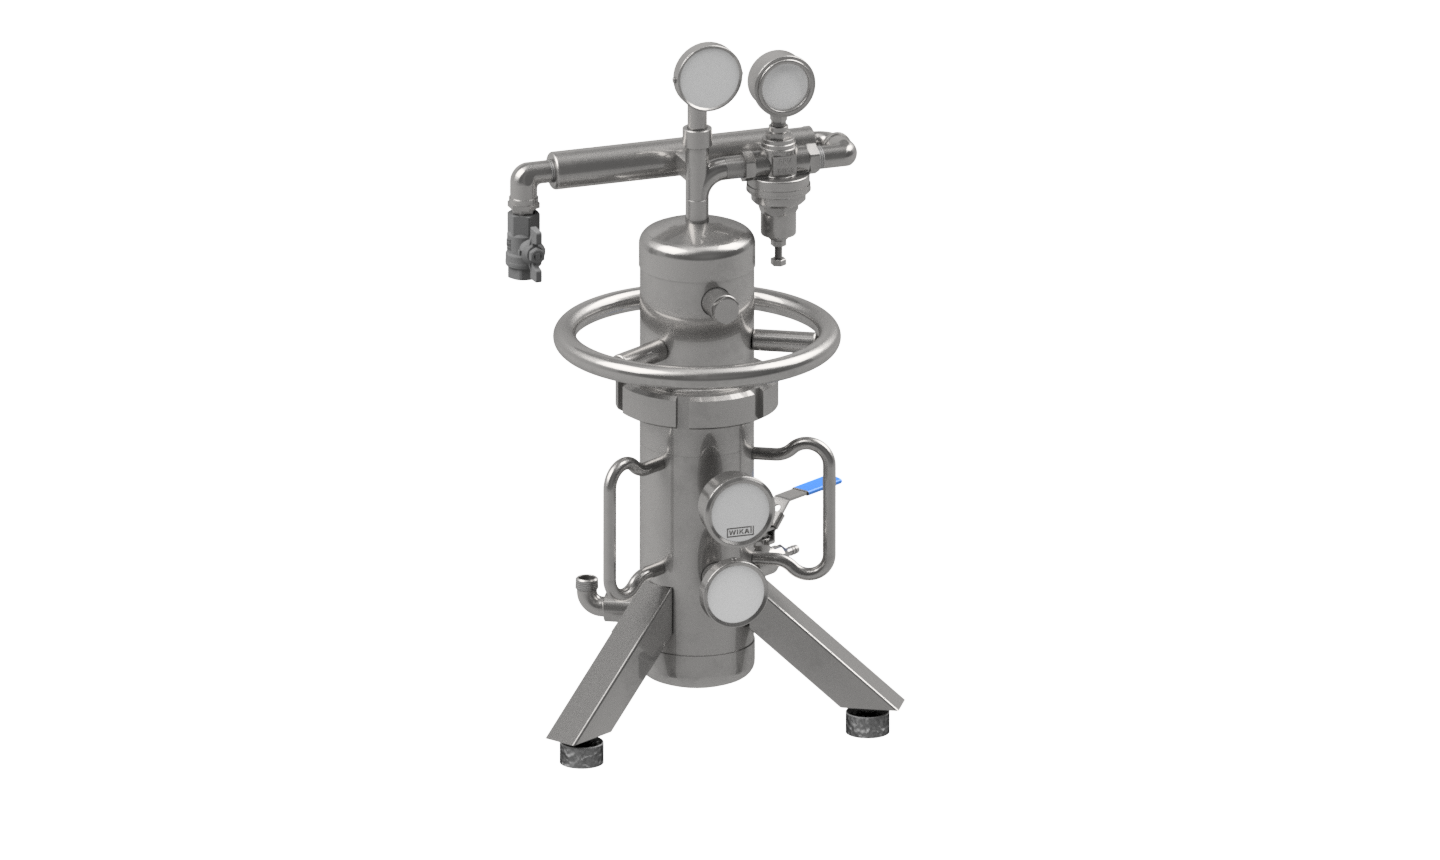
\includegraphics[keepaspectratio,width=\textwidth,height=\textheight]{render.png}
    \caption{3D Darstellung des Dampfdruckbehälters}\label{fig:render}
\end{figure}

\par

Dies ist auch in Abbildung \ref{fig:render} sehr gut zu erkennen (vgl. Abb.\ref{fig:render}).

\blindtext[2] \par


\subsection{Wahl der Dichtmittel}
\blindtext[2] \par

\subsection{Einflussgrößen auf die Auslegung nach AD2000}
\blindtext[1]

\begin{table}[htb]
\centering
\begin{tabular}{|c|cc|}
    \hline
 Einheit & Benennung & Kategorie \\
 \hline
 m & 6 & 8783 \\ 
 s & 7 & 78 \\
 V & 545 & 778\\
 A & 545 & 18744\\
\hline
\end{tabular}
\caption{Eine sehr vielaussagende Tabelle}\label{vielaussagend}
\end{table}

\blindtext[1]

\section{Formeln}
\begin{equation}
   a=b
    \label{eq:Eq3}
\end{equation}


\newpage
 
\begin{align}
\intertext{ Zum einen gilt: } 
a+b&=c
\intertext{zum anderen jedoch auch } 
b=c
\end{align}

Also was ist folglich c?


\begin{equation}\label{eq:Eq7}
   a=b
\end{equation}



\begin{equation*}\label{eq:Eq2}
   b=c
\end{equation*}

\begin{equation}
    \label{eq:Eq10}
    Y=Kd \ast \left(Xd + \frac{1}{Tn} + \int Xd\ dt + d\ \frac{Xd}{dt}\right)
\end{equation}



\newpage
\section{Fazit und sicherheitstechnische Beurteilung der Facharbeit}
\blindtext[1]\par\blindtext[1.2]





\end{document}

